\documentclass[12pt, twoside]{article}
\usepackage[letterpaper, margin=1in, headsep=0.5in]{geometry}
\usepackage[english]{babel}
\usepackage[utf8]{inputenc}
\usepackage{amsmath}
\usepackage{amsfonts}
\usepackage{amssymb}
\usepackage{tikz}
\usetikzlibrary{quotes, angles}

\usepackage{pgfplots}
\pgfplotsset{width=9cm,compat=1.9}
\usepgfplotslibrary{statistics}
\usepackage{pgfplotstable}

\usepackage{venndiagram}

\usepackage{graphicx}
\usepackage{enumitem}
\usepackage{multicol}
\usepackage{hyperref}

\newif\ifmeta
\metatrue %print standards and topics tags

\title{Pre-Calculus}
\author{Chris Huson}
\date{December 2022}

\usepackage{fancyhdr}
\pagestyle{fancy}
\fancyhf{}
\renewcommand{\headrulewidth}{0pt} % disable the underline of the header
\raggedbottom


\fancyhead[LE]{\thepage}
\fancyhead[RO]{\thepage \\ Name: \hspace{4cm} \,\\}
\fancyhead[LO]{BECA / PreCalculus-6. Descriptive Statistics\\* 15 December 2022}

\begin{document}

\subsubsection*{6.12 Quiz: Box and whisker plots}
\begin{enumerate}
\item Find the mean of the following set of numbers:
  \begin{center}
    9, 10, 14, 15, 17
  \end{center} \vspace{2cm}
  
\item Draw a box and whiskers plot of the five-figure summary on the grid. Use a ruler for full credit. \vspace{0.25cm}\\
min = 4, $Q_1=6$, median = 10, $Q_3=12$, maximum = 17
  \begin{center}
    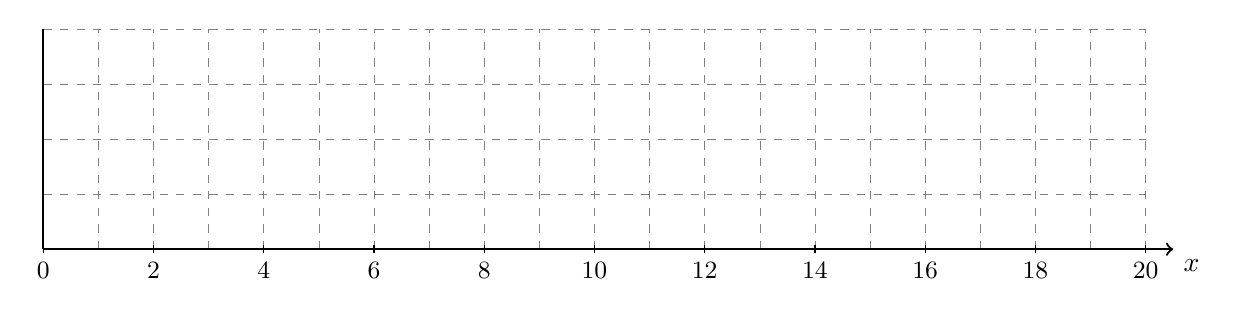
\begin{tikzpicture}[scale=.7]
      \draw [help lines, dashed] (0,0) grid (20,4);
      \draw [thick, ->] (0,0) -- (20.5,0) node [below right] {$x$};
      \foreach \x in {0,2,4,6,8,10, 12, 14, 16, 18, 20}
        \draw[shift={(\x,0)},color=black] (0pt,2pt) -- (0pt,-2pt) node[below] {\small $\x$};
      \draw [thick, -] (0,0)--(0,4);
    \end{tikzpicture}
  \end{center}

\item The box-and-whisker plot represents the examination scores of a group of students.
  \begin{center}
  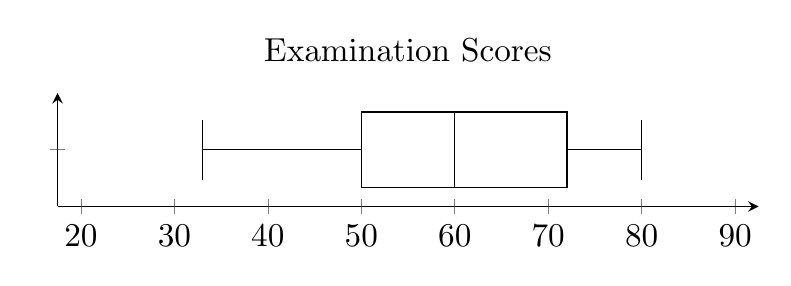
\begin{tikzpicture}[scale=1.2]
    \begin{axis}[
        title={Examination Scores},
        axis lines=left,
        xmin=30, xmax=80,
        y=1cm,
        ytick={1},
        yticklabels={},
      enlargelimits=0.25,
        ]
        %\addplot+ [boxplot]
        %table {3-11_IB-exam.txt};
       \addplot [boxplot prepared={draw position=1,
            lower whisker=33, lower quartile=50,
            median=60,
            upper quartile=72, upper whisker=80,
            %average=28,
            },
        ] coordinates {};
    \end{axis}
    \end{tikzpicture}
  \end{center}
  \begin{enumerate}
    \item Write down each value:
    \begin{enumerate}
      \begin{multicols}{3}
        \item median =
        \item $Q_1 = $
        \item max =
      \end{multicols}
    \end{enumerate} \vspace{0.5cm}
    The range of the scores is 47 marks, and the interquartile range is 22 marks. \vspace{0.5cm}
    \item Find the value of
    \begin{enumerate}
      \item the minimum score; \vspace{1cm}
      \item the third quartile. 
    \end{enumerate}
  \end{enumerate}


\end{enumerate}
\end{document}